\documentclass[arhiv]{../izpit}
\usepackage{fouriernc}
\usepackage{xcolor}
\usepackage{tikz}

\begin{document}

\izpit{Programiranje I: 1.\ izpit}{24.\ januar 2018}{
  Čas reševanja je 180 minut.
  Veliko uspeha!
}

%%%%%%%%%%%%%%%%%%%%%%%%%%%%%%%%%%%%%%%%%%%%%%%%%%%%%%%%%%%%%%%%%%%%%%
\naloga[]

\podnaloga
  Definirajte funkcijo \verb|izpisi_vsa_stevila|, ki sprejme seznam celih števil
  in zaporedoma izpiše vse njegove elemente.

  \begin{verbatim}
    # izpisi_vsa_stevila [1; 2; 3; 4];;
    1234- : unit = ()
    # izpisi_vsa_stevila [];;
    - : unit = ()
  \end{verbatim}

\podnaloga
  Definirajte funkcijo \verb|map2_opt|, ki sprejme funkcijo dveh argumentov
  in dva seznama. Vrne naj seznam rezultatov, ko dano funkcijo zaporedoma
  uporabimo na istoležnih elementih seznamov. Funkcija naj vrne rezultat le,
  kadar sta oba vhodna seznama enake dolžine, zato uporabite tip \verb|option|.
  %
  \begin{verbatim}
    # map2_opt (+) [1; 2; 3] [7; 5; 3];;
    - : int list option = Some [8; 7; 6]

    # map2_opt (+) [1; 2; 3] [7; 5];;
    - : int list option = None
  \end{verbatim}
  %
  Za maksimalno število točk naj bo funkcija \textbf{repno rekurzivna}.


%%%%%%%%%%%%%%%%%%%%%%%%%%%%%%%%%%%%%%%%%%%%%%%%%%%%%%%%%%%%%%%%%%%%%%
\naloga[]

\emph{Filtracijsko drevo} ima dve vrsti osnovnih gradnikov:
\begin{itemize}
\item Vozlišča imajo celoštevilsko vrednost, levo poddrevo in desno poddrevo.
\item Listi oz. škatle vsebujejo seznam celoštevilskih vrednosti.
\end{itemize}

\podnaloga
  Definirajte tip filtracijskih dreves \verb|filter_tree| ter
  drevo \verb|primer : filter_tree|, ki predstavlja sledeče filtracijsko drevo:
\[
  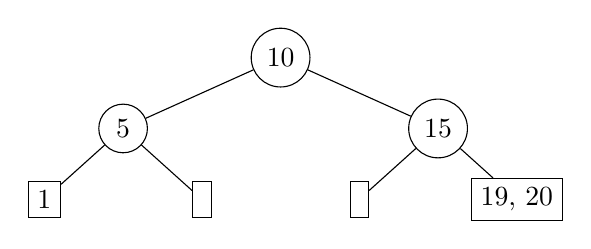
\begin{tikzpicture}[level distance=0.9cm,
    level 1/.style={sibling distance=4cm},
    level 2/.style={sibling distance=2cm},
    level 3/.style={sibling distance=2cm}
    ]
    \node[circle, draw] {10}
      child {node[circle, draw] {5}
        child {node[rectangle, draw] {1}}
        child {node[rectangle, draw] {\vphantom{1}}}
      }
      child {node[circle, draw] {15}
        child {node[rectangle, draw] {\vphantom{1}}}
        child {node[rectangle, draw] {19, 20}}
      };
  \end{tikzpicture}
\]


\podnaloga
  Filtracijsko drevo razvršča števila v škatle glede na njihovo vrednost.
  Vozlišče z vrednostjo $k$ razvrsti število $n$ v levo poddrevo, če velja
  $n \leq k$, oz.\ v desno poddrevo, če velja $n > k$.
  Ko število doseže škatlo, ga dodamo v seznam števil v škatli.
  Škatle lahko vsebujejo ponovitve in niso nujno urejene.

  Napišite funkcijo \verb|vstavi|, ki sprejme število in filtracijsko drevo in
  vrne filtracijsko drevo z vstavljenim številom.
  Na primer, \verb|vstavi 12 primer| vrne drevo:
  \[
    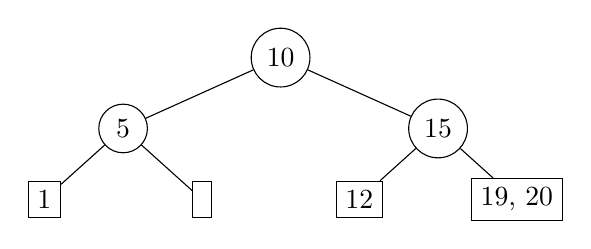
\begin{tikzpicture}[level distance=0.9cm,
      level 1/.style={sibling distance=4cm},
      level 2/.style={sibling distance=2cm},
      level 3/.style={sibling distance=2cm}
      ]
      \node[circle, draw] {10}
        child {node[circle, draw] {5}
          child {node[rectangle, draw] {1}}
          child {node[rectangle, draw] {\vphantom{1}}}
        }
        child {node[circle, draw] {15}
          child {node[rectangle, draw] {12}}
          child {node[rectangle, draw] {19, 20}}
        };
    \end{tikzpicture}
  \]

\podnaloga
  Napišite funkcijo \verb|vstavi_seznam|, ki sprejme seznam celih števil in
  filtracijsko drevo ter vrne filtracijsko drevo z vstavljenimi elementi seznama.
  Vrstni red vstavljanja ni pomemben.

\podnaloga
  Definirajte funkcijo, ki sprejme filtracijsko drevo in preveri, ali
  so vsa števila v pravilnih škatlah glede na način razvrščanja.
  Na primer, v levem drevesu so števila razvrščena pravilno, v desnem pa ne:
  \[
    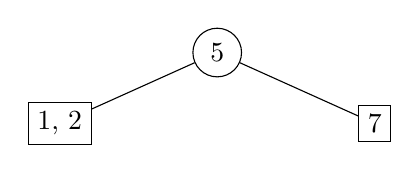
\begin{tikzpicture}[level distance=0.9cm,
      level 1/.style={sibling distance=4cm},
      level 2/.style={sibling distance=2cm}
      ]
      \node[circle, draw] {5}
        child {node[rectangle, draw] {1, 2}}
        child {node[rectangle, draw] {7}};
    \end{tikzpicture}
    \hspace{15mm}
    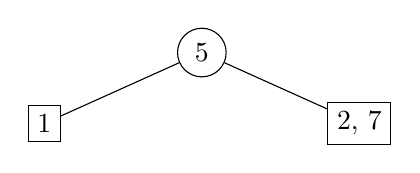
\begin{tikzpicture}[level distance=0.9cm,
      level 1/.style={sibling distance=4cm},
      level 2/.style={sibling distance=2cm}
      ]
      \node[circle, draw] {5}
        child {node[rectangle, draw] {1}}
        child {node[rectangle, draw] {2, 7}};
    \end{tikzpicture}
  \]

%%%%%%%%%%%%%%%%%%%%%%%%%%%%%%%%%%%%%%%%%%%%%%%%%%%%%%%%%%%%%%%%%%%%%%
\naloga[]
  Linearne preslikave na $\mathbb{Z}^2$ lahko predstavimo tako z matrikami kot s
  funkcijami, obe predstavitvi pa zadoščata signaturi \verb|Linearna|, ki določa:
  \begin{itemize}
  \item \verb|type t| --- tip linearnih preslikav;
  \item \verb|val id : t| --- identiteta;
  \item \verb|val uporabi : t -> vektor -> vektor| --- dano preslikavo uporabi na vektorju;
  \item \verb|val iz_matrike : matrika -> t| --- vrne linearno preslikavo, določeno z matriko;
  \item \verb|val iz_funkcije : (vektor -> vektor) -> t| --- vrne linearno preslikavo, določeno s funkcijo (predpostavite lahko, da je funkcija linearna);
  \item \verb|val kompozitum : t -> t -> t| --- vrne kompozitum danih preslikav.
  \end{itemize}
  %
  Pri tem vektorje in matrike predstavimo s pari oz.\ četvorci celih števil:
  \[
  \begin{bmatrix}
      x \\
      y
  \end{bmatrix}
  =
  (x, y)
  \hspace{5mm}
  \begin{bmatrix}
      a & b \\
      c & d
  \end{bmatrix}
  =
  (a, b, c, d)
  \]
  %
  Tako definiramo tipa

  \begin{verbatim}
    type vektor = int * int
    type matrika = int * int * int * int
  \end{verbatim}


\podnaloga
  Napišite modul \verb|Matrika : Linearna|, ki linearne preslikave predstavi
  z matrikami tipa \verb|matrika|.

\podnaloga
  Napišite modul \verb|Funkcija : Linearna|, ki linearne preslikave predstavi
  s funkcijami tipa \verb|vektor -> vektor|.

%%%%%%%%%%%%%%%%%%%%%%%%%%%%%%%%%%%%%%%%%%%%%%%%%%%%%%%%%%%%%%%%%%%%%%
\naloga[Nalogo lahko rešite v OCamlu ali Pythonu]

Lisjaček krade jabolka v sadovnjaku, kjer so jablane razporejene v vrstah.
Okrade lahko zgolj $N$ jablan, preden ga prežene lastnik sadovnjaka.

Ker je lisjaček še mlad in nevešč kraje jabolk, v vsaki vrsti obira
jablane eno za drugo in pri tem nobene ne preskoči. Ko se odloči, da se bo
lotil naslednje vrste, se ne vrne več nazaj. V primeru, da se znajde na koncu
zadnje vrste, svojo pustolovščino zaključi, ne glede na to, koliko časa mu je še preostalo.

Sadovnjak predstavimo z matriko, kjer vrstice predstavljajo
vrste sadovnjaka, vrednosti pa števila jabolk na jablanah.
Pri tej predstavitvi se lisjaček v vsakem koraku premakne bodisi v desno bodisi
na začetek naslednje vrstice.

\podnaloga
  Napišite algoritem, ki \textbf{učinkovito} izračuna največje število jabolk, ki jih lisjaček
  lahko ukrade. Na primer, če je $N = 6$ in je sadovnjak oblike
  \[
  \begin{bmatrix}
      2 & 4 & 1 & 1 \\
      3 & 2 & 0 & 5 \\
      8 & 0 & 7 & 2
  \end{bmatrix}\,,
  \]
  lahko lisjaček ukrade največ $24$ jabolk, kar stori tako, da izbere sledeče jablane:
  \[
  \begin{bmatrix}
      \textbf{2} & \textbf{4} & 1 & 1 \\
      \textbf{3} & 2 & 0 & 5 \\
      \textbf{8} & \textbf{0} & \textbf{7} & 2
  \end{bmatrix}
  \]

  \podnaloga
  V komentarju napišite in utemeljite časovno zahtevnost vašega algoritma.

\end{document}
